% !TeX spellcheck = <none>
\chapter{Visual Narrative}\label{sec-design}
Given the proliferation of data-driven storytelling in practice, it is of great importance to advance researches in visualization to identify factors that make visual data stories compelling and improve their performance in return. This chapter introduces existing works that focus on visual design in data-driven narratives. According to the role each work mainly serves in the storytelling process, we divide them into three categories, namely, scene, sequence, and transition. Considering a well-known principle in the design field, namely, "form follows function" \cite{form}, we then discuss main forms of visual narrative design and their corresponding functions in each category as shown in Table \ref{tab:story-component}. The representative works are describe in detail with both benefits and drawbacks. 
%In each category,we then describe the representative works in detail and discuss their benefits and drawbacks. 
%Based on this taxonomy, we also analyze a sample of existing visual data stories collected from online sources in Table []. 
Based on this taxonomy, we review current visualizaiton genres and  reflect on how they compose a visual data story.

\renewcommand{\arraystretch}{1.5}

\begin{table}[H]
	\centering
	\begin{tabular}{|l|c|l|l|}
		\hline
		\multicolumn{2}{|l|}{Categories}                                                                          & Form                        & Function                                                                             \\ \hline
		\multirow{13}{*}{\begin{tabular}[c]{@{}l@{}}Story\\ Component\end{tabular}} & \multirow{5}{*}{Scene}      & Close-up,~\cite{Furnas1986}                    & \multirow{2}{*}{Highlight}                                                           \\ 
		&                             & Change graphical properties~\cite{Waldner2014} &                                                                                      \\ \cline{3-4} 
		&                             & Text~\cite{Hullman2013, Gao2014, Ren2017}                        & Annotation                                                                           \\ \cline{3-4} 
		&                             & Pictogrphics~\cite{Goffin2017, Wang2018}                & Visual                                                                               \\ \cline{3-4} 
		&                             & Scale~\cite{Qu2018}                       & Consistency                                                                          \\ \cline{2-4} 
		& \multirow{3}{*}{Sequence}   & Timeline~\cite{Brehmer2017}                    & Navigation                                                                           \\ \cline{3-4} 
		&                             & Linear narrative,~\cite{Hullman2013a, Hullman2017, Kim2017a}            & \multirow{2}{*}{Structure}                                                           \\ 
		&                             & Non-linear narrative~\cite{Bach2018, Kim2018}        &                                                                                      \\ \cline{2-4} 
		& \multirow{5}{*}{Transition} & Camera motions~\cite{Wijk2004},              & \multirow{5}{*}{\begin{tabular}[c]{@{}l@{}}Linking\\ separated\\ scenes\end{tabular}} \\ 
		&                             & Static transition ~\cite{Robertson2008},           &                                                                                      \\ 
		&                             & Animated transition~\cite{Chevalier2014, Dragicevic2011, Elmqvist2008a, Guilmaine2012, Heer2007, Plaisant2002},         &                                                                                      \\ 
		&                             & Morphing~\cite{Drucker2015},                    &                                                                                      \\ 
		&                             & Metaphor~\cite{Huron2013, Lin2013, Wang2016},                    &                                                                                      \\ \hline
	\end{tabular}
\caption{Visual design in data-driven storytelling. In the \textit{Form} column, we list forms used in the related papers. The \textit{Function} column list the role the corresponding form serves.}
\label{tab:story-component}
\end{table}

%\renewcommand{\arraystretch}{1.3}

%\begin{table}[H]
%	\centering
%	\begin{tabular}{ |c|c|c|p{15em}|p{7.5em}| } 
%		\hline
%		\multicolumn{3}{|c|}{Categories} & Form & Function \\
%		\hline
%		\multirow{15}{6em}{\centering Story Component} & \multicolumn{2}{|c|}{\multirow{5}{6em}{\centering Scene}}
%		& Close-up, & \multirow{2}*{Highlight} \\
%		& \multicolumn{2}{|c|}{} & Change graphical properties & \\ 
%		\cline{4-5}
%		& \multicolumn{2}{|c|}{} & Text Narration  & Annotation \\ 
%		\cline{4-5}
%		& \multicolumn{2}{|c|}{} & kNNs & instance-based \\ 
%		\cline{2-5}
%		& \multicolumn{2}{|c|}{\multirow{5}{6em}{\centering Sequence}}
%		& Decision Trees, & \multirow{3}*{simplification} \\
%		& \multicolumn{2}{|c|}{} & Sparse SVMs , & \\
%		& \multicolumn{2}{|c|}{} & Sparse CNNs  & \\
%		\cline{4-5}
%		& \multicolumn{2}{|c|}{} & Sparsity by Bayesian , & \multirow{2}*{direct-sparsity} \\
%		& \multicolumn{2}{|c|}{} & Integer Models & \\
%		\cline{2-5}
%		& \multicolumn{2}{|c|}{\multirow{5}{6em}{\centering Transition}}
%		& Decision Trees, & \multirow{3}*{rule-based} \\
%		& \multicolumn{2}{|c|}{} & Rule Lists , & \\ 
%		& \multicolumn{2}{|c|}{} & Rule Sets & \\ 
%		\cline{4-5}
%		& \multicolumn{2}{|c|}{} & Linear Models  & linear \\ 
%		\cline{4-5}
%		& \multicolumn{2}{|c|}{} & kNNs & instance-based \\ 
%		\cline{2-5}
%		\hline
%	\end{tabular}
%	\caption{Visual design in data-driven narratives.}
%	\label{tab:story-component}
%\end{table}

\section{Scene}
One of the important components in data-driven storytelling is visual design in scenes, which aims to communicate events and facts in conjunction with data to a broad audience. Qualified visual representations are supposed to describe data and amplify cognition. With a curated collection of visualization artifacts online, some researchers conducted surveys to extract techniques and inform the design space.

Segel and Heer ~\cite{Segel2010} took an initial step in classifying techniques and formulating the design from an analysis of 58 examples, as was mentioned in Section 2.2. This kind of work has shed light on further research in narrative visualization. Hullman and Diakopoulos ~\cite{Hullman2011} expanded their discussion including extra-representational influencers like contextual differences in interpretation. They distinguished four editorial layers for conveying meaning, which covered the whole creation process from the data, visual representation, textual annotation, to interactivity. Based on an observation of 51 professionally-produced narrative visualizations, five major forms of rhetorical techniques were identified in this genre of storytelling, namely, information access rhetoric, provenance rhetoric, mapping rhetoric, procedural rhetoric, and linguistic rhetoric. Specifically, these strategies of visualization rhetoric worked as an analytical framework to understand how visual techniques could prioritize particular interpretations. Since then, Stolper et al. ~\cite{Stolper2016} also adopted this empirical approach to enrich the range of techniques in constructing scenes, such as textual and audio narration, text annotation, labeling, and tooltips, and show their evolution over time. While many of these surveys investigate data stories but are agnostic to the data type, Brehmer et al. ~\cite{Brehmer2017} provided a detailed analysis which is specific to timelines describing from three dimensions, namely, representation, scale, and layout. Thus, several fundamental elements embellishing scenes have been recognized through multiple iterations, such as annotations, representation, and highlights.

Although extracting design guidance by empirical studies is deemed as a feasible approach, it faces several problems.  The design knowledge is derived from a small sample of visualization examples and is also continually evolving, thus leading to the incompleteness \cite{Moritz2018}. And there exists inevitable subjectivity when grouping and summarizing techniques. Apart from conducting surveys to inform the design space, the visualization research community has proposed new methods to optimize the scene representations recently. 

Nearly all the above surveys argued that text \textbf{annotations} play an important role in supplementing visualization and directing readers' attention. Many efforts have been made to create annotated information visualizations for online news \cite{Hullman2013, Gao2014}. Hullman et al. \cite{Hullman2013} proposed the Contexifier system targeting at providing context for business news as shown in Figure \ref{Contexifier}. It first automatically creates a timeline graph of one company’s stock. Other articles with relevant contents about this company feed information to the additive customized annotations for the line graph visualization. The selection and layout of those annotations in the graph depended on an underlying algorithm in view of three factors, namely, linguistic relevancy of the topic, visual saliency based on the data series, and analysis of article volume about historical events. 

\begin{figure}[htb]
	\centering 
	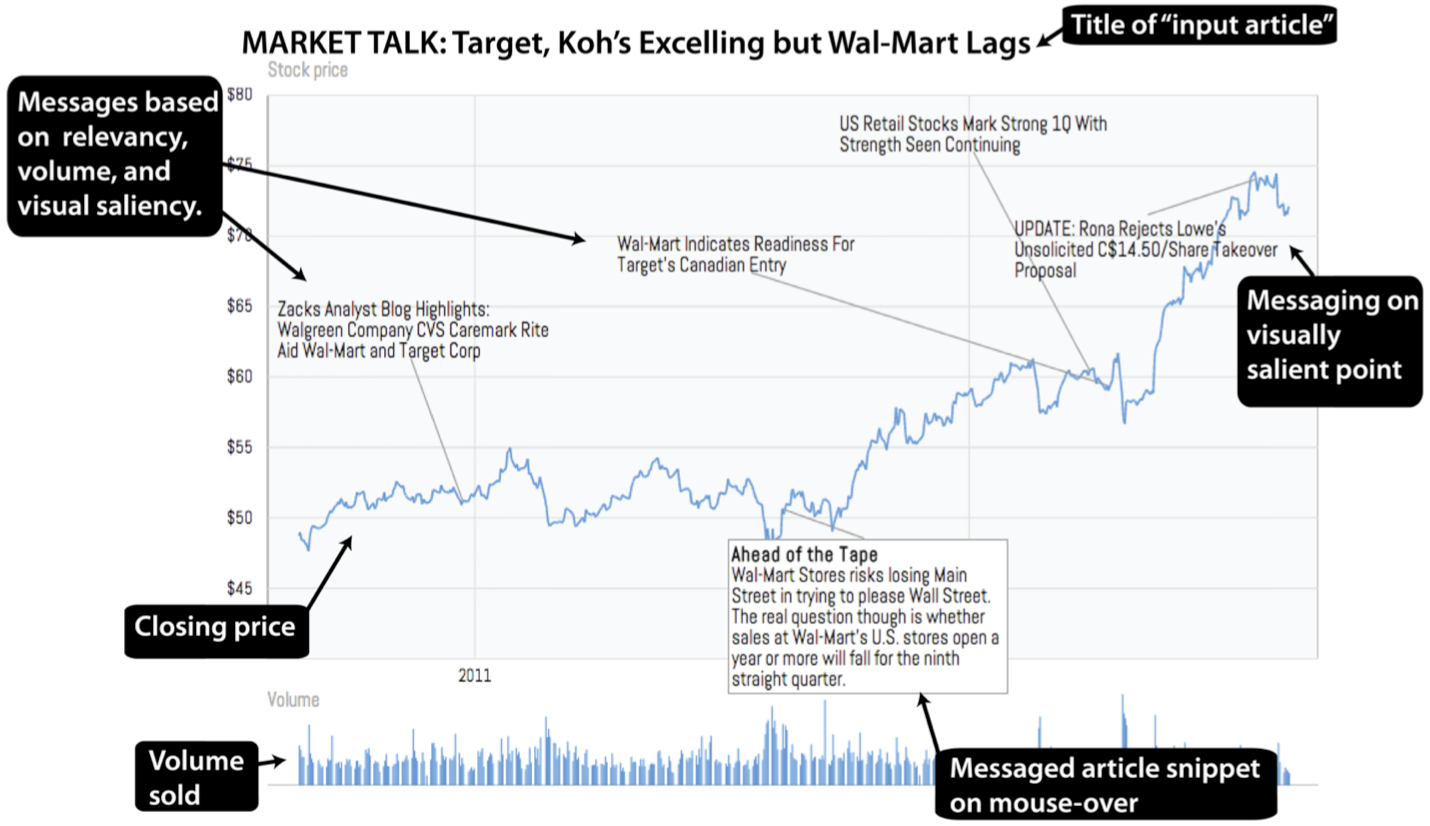
\includegraphics[width=0.95\textwidth]{figure/contiexifier.png} 
	\caption{ An annotated visualization produced by Contextifier \cite{Hullman2013}. } 
	\label{Contexifier} 
\end{figure}

Since Contextifier takes a step towards annotated news visualization but is limited to the stock time series using line charts, Gao et al. \cite{Gao2014} further contributed a news generation pipeline to this area. 
%As shown in Figure \ref{pipeline}, this pipeline negotiated six main points based on an abundant news corpus. 
And the NewsView system implemented this pipeline to automatically generate interactive and annotated maps, which was the most prevalent form of these visualization. 

In addition to automated generation, Ren et al. \cite{Ren2017} developed ChartAccent, an authoring tool that allows users to augment charts with annotations easily. The current system provided manual and data-driven annotations based on the design space informed by 106 annotated charts. However, the problem in the reproduction study is that default data-driven annotations were not ideal most times. It reflects on the challenge that the initial design space might be incomprehensive, leading to the ineffectiveness of the tool.

Among a variety of narrative visualizations, most rely on a few basic visualization forms, such as the above line graphs, bar charts, and maps, as well as \textbf{infographics} (also known as pictographs) \cite{Amini2015}. Some researches \cite{Amini2018} also attest to the prominence of pictographic representation by triggering viewers' engagement compared with standard charts through a crowd-sourced online study. Therefore, it attracted research interests in easing the creation of data-driven infographics \cite{Kim2017, Wang2018} and embedding them to provide compelling scenes \cite{Amini2017, Goffin2017}.

\begin{figure}[htb]
	\centering 
	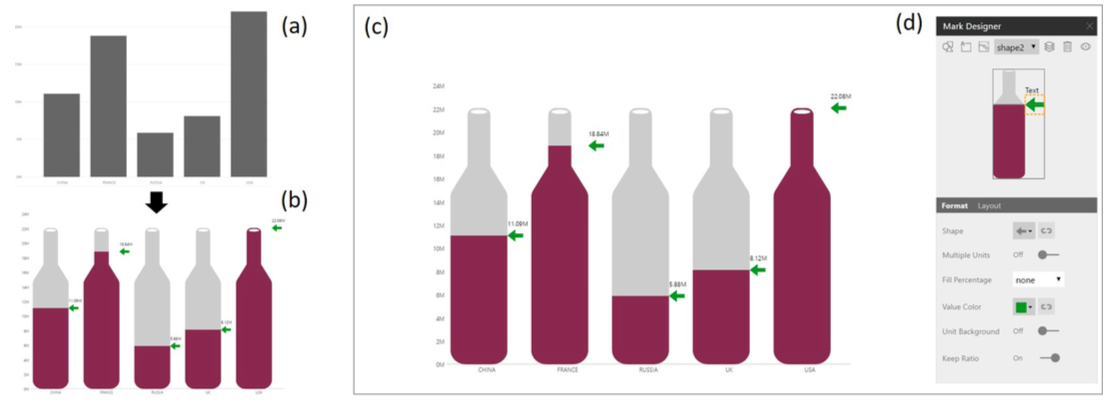
\includegraphics[width=0.98\textwidth]{figure/InfoNice.png} 
	\caption{A use case to change the original column chart to an infographic style version with customized marks with InfoNice \cite{Wang2018}. } 
	\label{InfoNice} 
\end{figure}


Another frequent technique adopted by authors when creating scenes is to perform element \textbf{highlighting}.  There are many methods found in visualization practices, such as wrapping highlighted items with a shape and fading out unessential parts to emphasize important ones. 
Waldner et al. \cite{Waldner2014} enhanced the focus to pop out from its context in a large dynamic scene using a strong visual attractor, flicker. Some movie narrative techniques could be used for reference in data-driven storytelling. For example, fisheye views \cite{Furnas1986} as a close-up highlight element details to the audience. 

Despite these promising design guidelines, an often-overlooked aspect is the wide existence of multiple views. Effective single views may constitute inconsistent multiple scenes, leading to slow and error-prone interpretation. Qu and Hullman presented a qualitative study to investigate specific \textbf{consistency} constraints and exceptions \cite{Qu2018, Qu2016}. As shown in Figures \ref{Consistent}, there were more validations than exceptions considering constrains specialized to scales (e.g., color scale, x or y scale).  The exceptions indicated conditions where specific design rationales should defend inconsistencies and override constraints. These findings provided a foundation for automated inconsistency detection mechanisms. Nevertheless, this work mainly started   from the perspective of authors to create multiple scenes and did not study the impacts inconsistency leave to viewers. 

\begin{figure}[htb]
	\centering 
	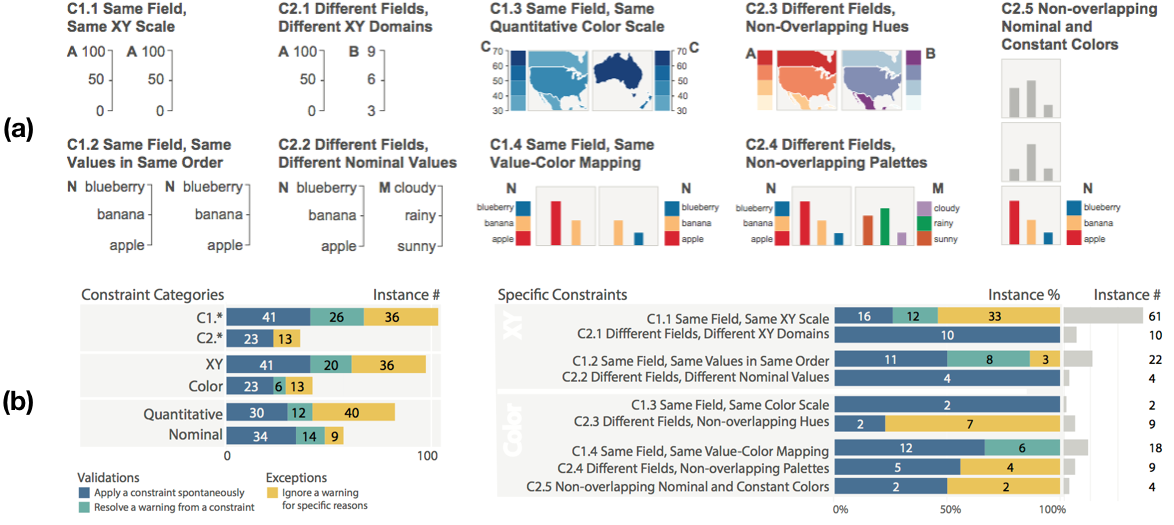
\includegraphics[width=0.98\textwidth]{figure/consistent1.png} 
	\caption{Qu and Hullman conducted quantative studies for XY and color scales to investigate consistency principle (a) and counted validation and exception (b) \cite{Qu2018}. } 
	\label{Consistent} 
\end{figure}


In summary, many surveys have identified basic elements and techniques from analysis of visualization artifacts. Several works develop tools to either ease the creation or augment representations. And the research community also begins to explore high-level design principles such as consistency to further embellish storytelling. However, the expressiveness and effectiveness are evaluated based on a small sample of both users and visualizations in most cases. And there remain research efforts to explore more design considerations. For example, audio narration like background music is indispensable in some narrative forms, but few works have advanced in this direction.

\section{Sequence}

Conveying a narrative with data visualization requires story creators to thread representations into a compelling yet understandable sequence. This form of author-specified ordering differentiates itself from open-ended explorations by providing navigation aids frequently with explicit structures. Several surveys ~\cite{Stolper2016, Segel2010} initialize and further enlarge a variety of techniques used in visualization artifacts to communicate structures and navigation to viewers. These techniques include next/previous buttons, scrolling, breadcrumbs, section header buttons, menu selection, timelines, and geographic maps. Besides, some works focus on the narrative structures. Based on Cohn's theory of visual narratives ~\cite{Cohn2013}, Amini et al. ~\cite{Amini2015} identified the structures from a qualitative analysis of 50 data videos, which consisted of four major narrative categories, i.e., Establisher (E), Initial (I), Peak (P), Release (R). An example with detailed explanation for each category is shown in Figure \ref{sequence1}. According to the findings, they noted that most data videos followed this method, and the Initial category played the most prominent role in data videos. 

\begin{figure}[htb]
	\centering 
	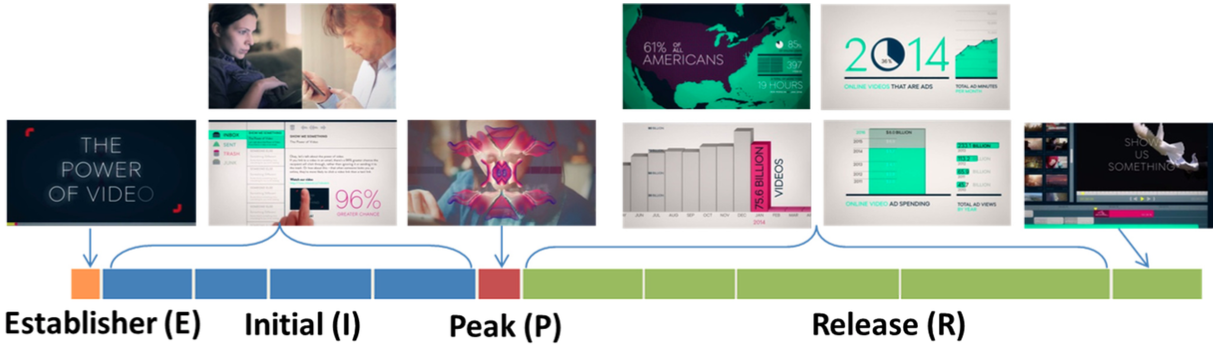
\includegraphics[width=0.98\textwidth]{figure/sequence1.png} 
	\caption{Visual narrative structures: \textit{Establisher} provides referential information; \textit{Initial} "sets the action or event in motion"; \textit{Peak} reflects on the most important events; and \textit{Release} shows "the aftermath of the Peak" \cite{Amini2015}. } 
	\label{sequence1} 
\end{figure}

Researches in the visualization community have studied this category in depth. Hullman et al. ~\cite{Hullman2013a} provided a deeper understanding of sequence in the form of linear, "slideshow-style" presentations. Starting from a qualitative analysis of 42 narrative visualizations, they gained insights on how to structure visualization storytelling. The first finding pointed out six transition types distinguished by changes to data dimensions and used to drive transformations between visualizations.  Another finding describes higher-level strategies that local transitions (visualization-to-visualization) respond to a small number of changes to data dimensions, while global transitions (involving multiple local transitions) are required to maintain consistency in the form of parallelism. These results helped them build a semi-automatic graph-driven approach for visualization sequence supports. An objective function is proposed with an aim to minimize the transition costs considering audience's perceptions. After that, Hullman et al. ~\cite{Hullman2017} further studied impacts that transitions bring to longer visualization sequences. Their results indicated a hierarchical structure preferred by humans beginning with grouping subsets of visualizations with shared data properties.

Based on these works, Kim et al. ~\cite{Kim2017a} presented GraphScape, a directed graph model to extend automated reasoning about visualization similarity and sequencing. Instead of a focus on conceptual transition types as Hullman et al. did, GraphScape leverages the Vega-Lite language and works on a more sophisticated cost function balancing local and global transitions. Thus, this model works both as a generative tool (e.g., given a started visualization, traverse the graph and provide a sequence for this series of visualizations) and an evaluation tool (e.g., given a sequence of visualizations, measure their costs). However, this work currently implements at a level of visualization specification and does not go deep into the data level. 

\begin{figure}[htb]
	\centering 
	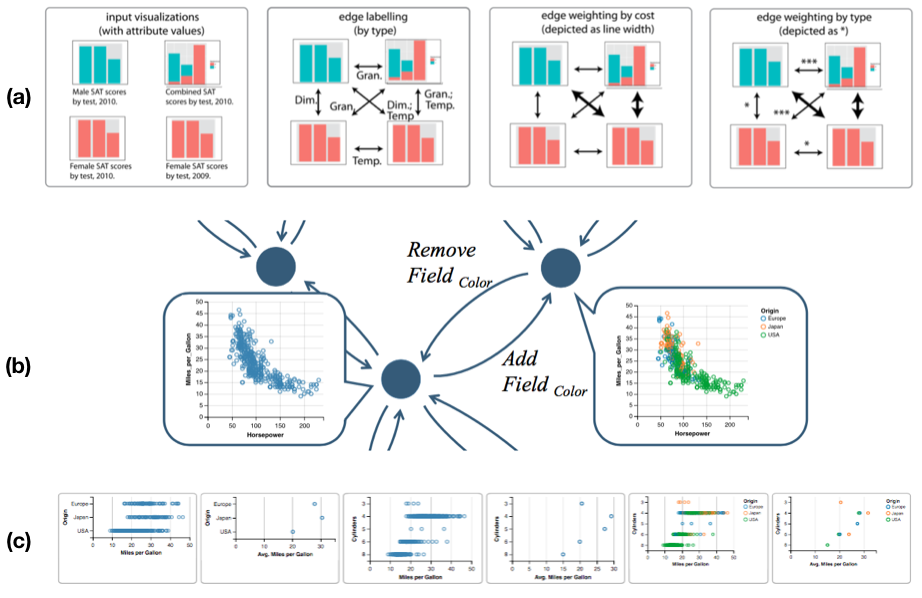
\includegraphics[width=0.98\textwidth]{figure/GraphScale2.png} 
	\caption{ (a) Diagram of the graph-based approach where each visualization represents a nodes and edges stand for possible transitions whose weights are calculated by the cost function \cite{Hullman2013a}. (b) The GraphScape model extended from (a) \cite{Kim2017a}. (c) An example of a viusalizaion sequence. } 
	\label{GraphScale} 
\end{figure}

However, above works all focus on linear sequences. In practice, narrative visualizations do not necessarily conform to the linear narration. For example, a well-received data video named "Wealth Inequality in America" ~\cite{inequality} does not adopt a linear narrative as well. It is based on comparisons among three conditions, i.e., the ideal condition, what American think, and the reality. Recently, Kim et al. ~\cite{Kim2018} presented Story Explorer to visualize non-linear narratives in movies. It provided a curated collection of non-linear narrative techniques, including flashbacks, flashforwards, bidirectional flashes, zigzags, follow-the-hero, and so on. Bach et al. \cite{Bach2018} identified flashback as a critical narrative in data comics. Wang et al. \cite{Wang2016} applied foreshadowing to present video clickstream data. However, most of them are not studied in the field of data-driven storytelling and few tools support to embed these techniques for visualization sequencing.

\section{Transition}

A narrative typically contains an account of multiple events or facts described in a series of ordered scenes. Linking these separated story scenes is crucial, especially providing transitions with attractive and engaging visual effects. Segel and Heer ~\cite{Segel2010} pointed out \textit{transition guidance} as an important dimension in visual narrative tactics. They found the common techniques in narrative visualization borrowed from films, e.g., camera motions, animated transitions. As such, much practice and research have studied this category in depth.  

\textbf{Camera motions} remain an ever-present mechanism in many visual data stories. The main advantage of imagining a virtual camera in data-driven narratives is its innate nature, as it conforms to the way how humans perceive the real world. Thus, it can easily elicit viewers' engagement by triggering their emotions. For example, in the "Global Wealth Inequality" video \cite{globalnequality}, when describing the richest 1\% have accumulated 43\% of our world's wealth, the authors moved the camera quickly along the bar but still took some time to reach the top. It easily provoked emotions and emphasized the wealth gap between the rich and the poor to the audience. In addition to camera viewing, other techniques such as zooming and panning are used frequently as well. Research in this area concentrates more on optimizing the smooth effects and is maturing rapidly.  For instance, Wijk and Nuij \cite{Wijk2004} presented a model to handle smooth viewing with a focus on simultaneous zooming and panning. However, the evaluation of the effect was based on the perception and did not consider the cognitive aspects which also played an important role in this kind of animation. 

\begin{figure}[htb]
	\centering 
	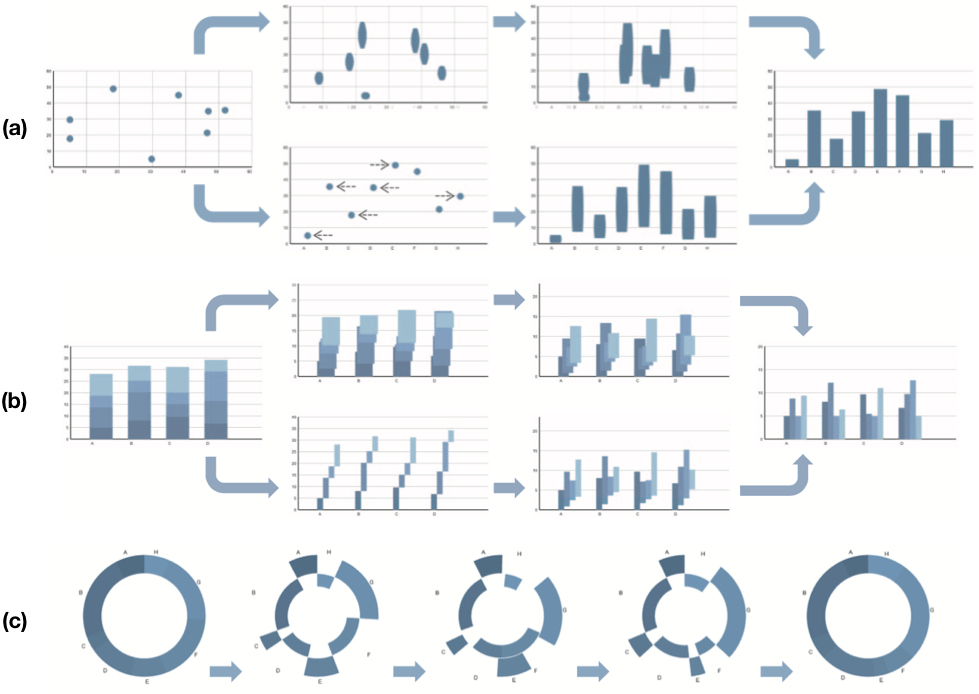
\includegraphics[width=0.98\textwidth]{figure/transition.png} 
	\caption{ Animated transitions between statistical data graphics. (a) Animating from a scatter plot to a bar chart. (b) Animating from stacked bars to grouped bars. (c) A multi-stage animation of changing values in a donut chart \cite{Heer2007}. } 
	\label{animated} 
\end{figure}

\textbf{Animated transitions} are another promising technique to connect story scenes and facilitate perception of changes between related data visualizations.  As a typical example like \textit{Green Honey} \cite{honey} shows, when viewers scroll down, the transitions will be triggered by small points' flying to their new position according to different colors. Heer and Robertson \cite{Heer2007} studied the design and effectiveness of animated transitions between statistical data visualizations such as bar charts, pie charts, and scatter plots as shown in Figure \ref{animated}. They crafted a taxonomy of seven transition types and proposed a visualization system, DynaVis for assessing the efficacy. The finding showed that animated transitions can improve graphical perception. However, not all animated transition scenarios are significantly different. For example, staged transitions only gain modest performance compared with linear transitions. Also, in this work, they just identified the design space among three common statistical data graphics and did not cover a wide range of transition scenarios. Some researches expand it to tree structures. Plasisant et al. \cite{Plaisant2002} proposed SpaceTree breaking the transition into 3 stages. Guilmaine et al. \cite{Guilmaine2012} further compared four animated transitions in a radial tree visualization, i.e., linear, staged, hierarchical, and a hybrid animation mixed with the staged and hierarchical approaches. The results indicate the hierarchical transitions in tree visualizations outperform other techniques significantly. However, the evaluation was just based on a target-tracking task and required to be further validated. Another research focus on animated transitions is to evaluate the effectiveness of  such techniques like temporal distortion \cite{Dragicevic2011} and staggering effects \cite{Chevalier2014} in visual tracking. The findings showed the benefits using these techniques, but the extent depended on the conditions and transition types.

Besides, animated transitions in \textbf{3D space} is much eye-catching. Some software like PowerPoint and Keynote has already embedded such transitions such as cube and box. Elmqvis et al. \cite{Elmqvist2008a} integrated animated rotations in 3D space, somewhat akin to rolling the dice, in scatterplot matrix navigation. 

\textbf{Morphing} is a special effect in animations which "changes one shape into another through a seamless transition" \cite{morphing}. This technique has been applied to several online visual data stories, such as EPFL Data Monolith \cite{EPFL} and The Rhythm of Food \cite{food}. They typically use points as basic elements. The previous data graphic is separated into multiple points, then these points animate to their new positions and form a new data visualization. Similarly, Drucker and Fernandez \cite{Drucker2015, Park2018} presented SandDance to explore the effectiveness of animating between unit representations as shown in Figure \ref{sandDance}.  

\begin{figure}[H]
	\centering 
	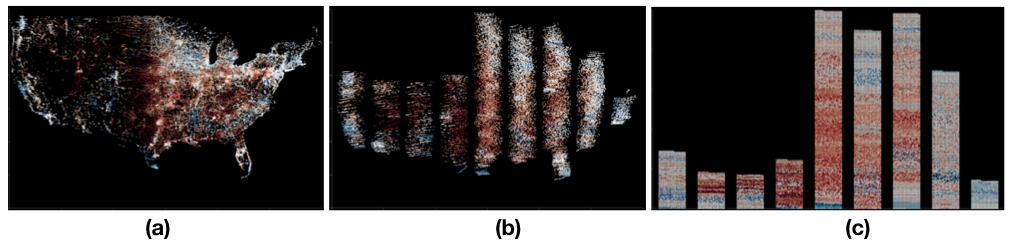
\includegraphics[width=0.98\textwidth]{figure/SandDance.png} 
	\caption{ A sequence explores the 2010 American election \cite{Drucker2015}. (a) Scatter plots are colored by voting percents on the map. (b) The path interpolates between the starting and ending states. (c) Bar charts are binned by logitude. } 
	\label{sandDance} 
\end{figure}

\textbf{Visual metaphors} show wonderful performance in data-driven storytelling and presentation but require much creativity. Visual Sedimentation \cite{Huron2013} presents an attractive design metaphor for visualizing data streams in Figure \ref{sedimentation}. It simulates the real-world sedimentation processes where objects fall because of gravity and then aggregate into strata over time. As for data streams which have incoming data continually, sedimentation fits a lot since data is encoded as objects and a force model controls the falling rate. Wang et al. \cite{Wang2016} also used this metaphor to visualize video clickstream data. Lin and Vuillemot \cite{Lin2013} explored spirograph designs for ambient display of Tweets. However, one problem for these visual metaphors is that they increase pressure for viewers to accurately extract the data. It might be not appropriate for strict data exploration.

\begin{figure}[htb]
	\centering 
	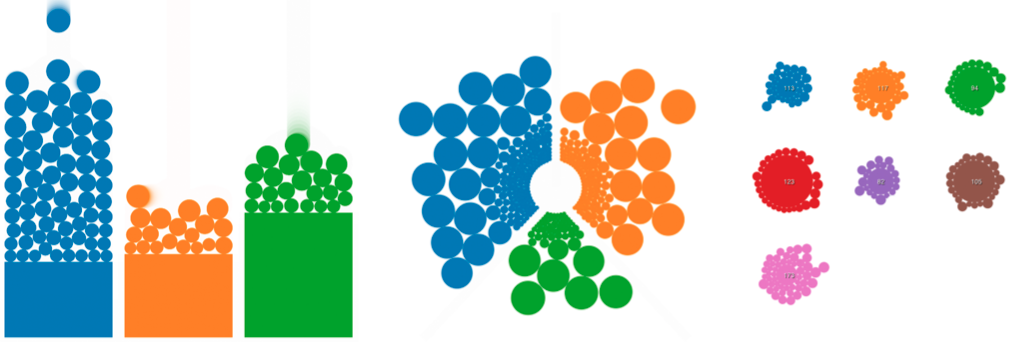
\includegraphics[width=0.95\textwidth]{figure/sedimentation.png} 
	\caption{ The Visual Sedimentation metaphor is applied to a bar chart (left), a pie chart (center), and a bubble chart (right) \cite{Huron2013}. } 
	\label{sedimentation} 
\end{figure}

Despite multiple animated transition techniques have been created and implemented in the visualization research, Amini et al. \cite{Amini2017} found such transitions are uncommon in data videos today. They suspected the complexity of realizing them with some programming skills and the lack of support in existing video editing tools contribute to the deficiency. Thus, they opted to support such kind of transitions as shown in Figuire \ref{lens}. However, they only extended  chart transitions \cite{Heer2007} to and from pictographs. Their finding  also indicated a gap that data visualization tools are not keeping up with the pace of innovations, as Google News Lab pointed out \cite{GoogleNews}. 

\begin{figure}[htb]
	\centering 
	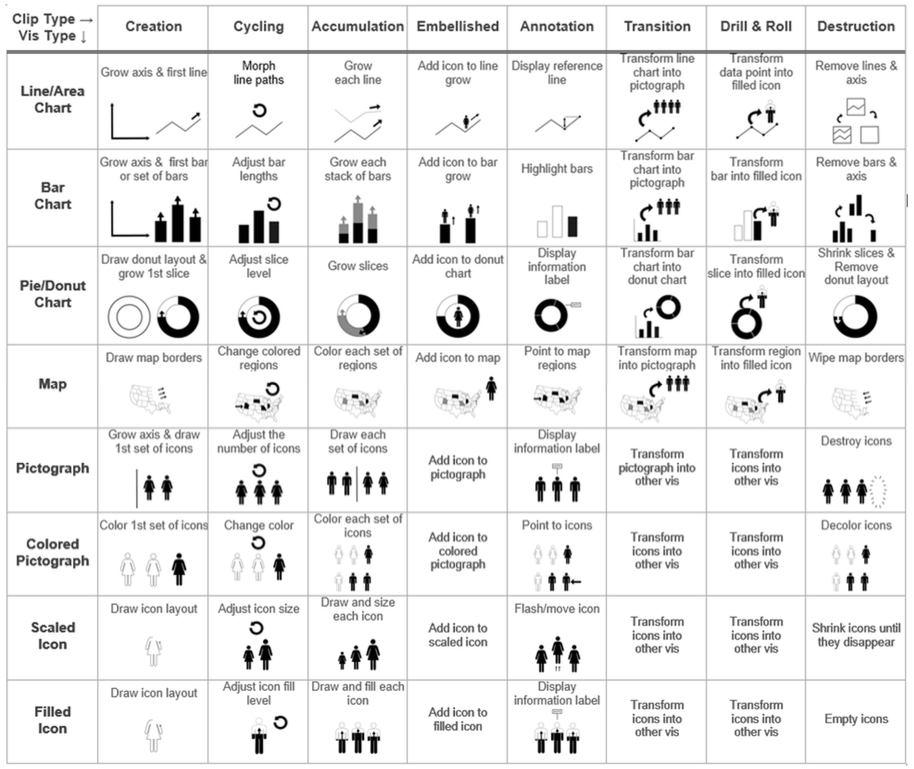
\includegraphics[width=0.95\textwidth]{figure/lens.png} 
	\caption{ Clip types as a function of  visualization types (rows)  and animation types  (columns) supported by DataClips \cite{Amini2017}. } 
	\label{lens} 
\end{figure}

However, the use of animation always arouses a heated discussion \cite{Fisher2010}. Robertson et al. \cite{Robertson2008} compared two alternative trend visualizations based on static representations in Figure \ref{trend} with the animated Gapminder Trendalyzer. The finding showed that trend animation can be challenging both in analysis and presentations. Although animations made participants enjoyable and exciting, it resulted in many errors. However, some works \cite{Amini2018, Heer2007} argued that animation can boost understandability of data insights and increase focused attention. Thus, without a series of unified evaluation criteria, it is hard to assess the effectiveness of visual data stories.

\begin{figure}[htb]
	\centering 
	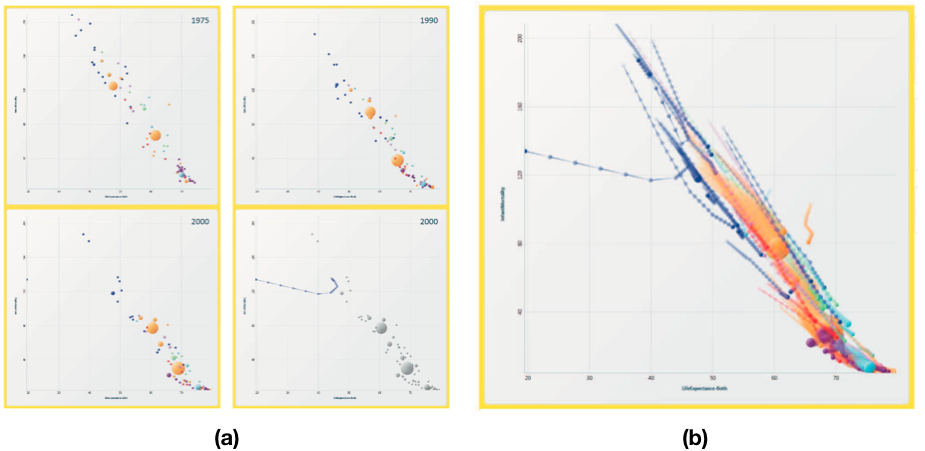
\includegraphics[width=0.95\textwidth]{figure/Trend.png} 
	\caption{ Two alternative static trend visulizations \cite{Robertson2008}. (a) A small multiples display the trend traces side by side. (b) One display shows traces of all trends overlaid simultaneously. } 
	\label{trend} 
\end{figure}


\section{Combining Multiple Components}

In the above sections, we identify three major components to compose a data-driven narrative, namely, scenes, sequences, and transitions. We learn from both research and practice to inform the design space of each component, respectively. Actually, a visual data story is not required to explicitly comprise all three parts. Take seven genres of narrative visualization (Figure \ref{taxonomy1}) for example. A magazine style which embeds visualization in a page of text or an annotated chart usually has a single frame. Thus, they may clearly address the scene design. The sequence and transition deal more with external factors such as text narration. Authors may consider the narrative sequence for the layout of partitioned posters ("multi-view visualizations"), flow charts, or comic strips, but are likely to employ a simple static transition between multiple frames. When authoring slide shows or film, these three components all play important roles. The scene design gives a basic representation to communicate data insights. The narrative sequence works for the goal of storytelling such as comparisons and trends, thus amplifying cognition. Advanced animated transition effects engage a broad range of viewers.

We also examine the story components with new emerging genres like ScrollyTelling \cite{scrollytelling} and SketchStory \cite{Lee2013}. First, ScrollyTelling asks viewers to scroll down to explore visual stories. It is similar to slide shows but provide more transition techniques such as scrolling interactions and animation effects. SketchStory spans annotated charts, partitioned posters, and videos. It allows authors to sketch along the real-time presentation with pen and touch interactions as shown in Figure \ref{sketchStory}. It enriches the storytelling with audio narration and real-time feedback.

\begin{figure}[htb]
	\centering 
	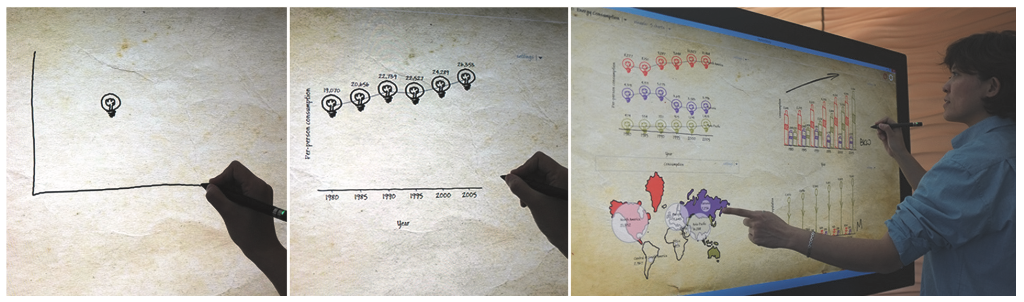
\includegraphics[width=0.95\textwidth]{figure/SketchStory.png} 
	\caption{ Telling a real-time story using SketchStory \cite{Lee2013}. } 
	\label{sketchStory} 
\end{figure}

However, we have seen that the proliferation of different narrative visualization genres and richness of techniques they employ in practice are largely limited to the authoring tools. Many research works have developed novel design and interactions. Most of them are not embedded into existing tools and require extra programming capabilities which practitioners tend not to equip with. 


\newpage